\hypertarget{ux4e16ux754c-ux52a8ux4f5cux6a21ux578b}{%
\chapter{世界-动作模型}\label{ux4e16ux754c-ux52a8ux4f5cux6a21ux578b}}

\hypertarget{ux4e16ux754c-ux52a8ux4f5cux6a21ux578bux6982ux8ff0}{%
\section{世界-动作模型概述}\label{ux4e16ux754c-ux52a8ux4f5cux6a21ux578bux6982ux8ff0}}

\hypertarget{ux4e00ux4e16ux754c-ux52a8ux4f5cux6a21ux578bux7684ux6982ux5ff5}{%
\subsection{一、世界-动作模型的概念}\label{ux4e00ux4e16ux754c-ux52a8ux4f5cux6a21ux578bux7684ux6982ux5ff5}}

世界-动作模型（World-Action Model，WAM）是世界模型范式在具身智能基础模型中的运用。世界-动作模型将状态预测和动作生成相结合，输入过去的状态（和已经采取的动作），用统一模型依次或同时预测下一状态和接下来的动作。其中，用统一模型是考虑到本质上都是在学习物理世界的规律，很多参数本就是重合的，且统一模型更符合端到端原则。

\hypertarget{ux4e8cux4e16ux754c-ux52a8ux4f5cux6a21ux578bux7684ux8badux7ec3ux76eeux6807}{%
\subsection{二、世界-动作模型的训练目标}\label{ux4e8cux4e16ux754c-ux52a8ux4f5cux6a21ux578bux7684ux8badux7ec3ux76eeux6807}}

WAM的损失函数一般为状态（视频像素或视觉特征）损失与动作损失加权求和：

\[
\mathcal{L}_{\mathrm{vid}}+\lambda_{\mathrm{act}}\mathcal{L}_{\mathrm{act}}
\]

两项大多采取流匹配损失：

对于目标变量 \(y\)（既可以是动作序列 \(a_{1:H}\)，也可以是未来视觉特征 \(z_{1:T}\)），算法采样高斯噪声 \(\varepsilon\sim\mathcal{N}(0,I)\) 和时间步 \(t\in(0,1)\)，构建插值样本：

\[
y_t=(1-t)y+t\varepsilon.
\]

模型通过标准的流匹配损失预测速度场：

\[
\mathcal{L}_{\mathrm{FM}}(y)=\mathbb{E}_{y,\varepsilon,t}\left[\left\|f_\theta(y_t,t,o,l)-(\varepsilon-y)\right\|_2^2\right].
\]

\hypertarget{ux4e09ux5177ux8eabux539fux751fux6a21ux578b}{%
\subsection{三、具身原生模型}\label{ux4e09ux5177ux8eabux539fux751fux6a21ux578b}}

早期的WAM往往由视频生成模型后训练得到。但视频生成模型本来是为数字内容创作而生，搬到机器人身上，会带来三个问题：

\begin{enumerate}
\def\labelenumi{\arabic{enumi}.}
\item
  表征的VAE只为像素级重建优化，宝贵的潜空间大半让给了光影、背景纹理和物体表面的高光，而杯子正在向左移动这种真正跟控制有关的事，只占极小的一部分。它保住了视觉细节，丢掉的恰恰是物理和语义结构。且动作模块往往是一个外挂部分，世界状态和动作被留在两个对不齐的空间里。
\item
  速度高维的视频token叠上多步迭代的去噪过程，延时长，而真机操作要求策略在每个动作块的边界上读入新观测、随时修正。
\item
  互联网视频没有动作标签，而通用的视频预测目标并不教模型``动作如何改变世界''。
\end{enumerate}

故现在许多WAM转向了用具身数据原生训练。这种方式对算力和数据要求更高，但模型能力的上限也更高。

\hypertarget{ux53c2ux8003ux6587ux732e-158}{%
\subsection{参考文献}\label{ux53c2ux8003ux6587ux732e-158}}

\vspace{0.25em}
\begin{itemize}
\tightlist
\item
  Wang, S., Shi, J., Fu, Z., et al.~(2026). \href{https://arxiv.org/abs/2605.12090}{World Action Models: The Next Frontier in Embodied AI}. arXiv:2605.12090.
\item
  Lipman, Y., Chen, R. T. Q., Ben-Hamu, H., Nickel, M., \& Le, M. (2023). \href{https://arxiv.org/abs/2210.02747}{Flow Matching for Generative Modeling}. ICLR.
\end{itemize}

\clearpage

\hypertarget{ux4e16ux754c-ux52a8ux4f5cux7edfux4e00ux751fux6210ux6a21ux578b}{%
\section{世界-动作统一生成模型}\label{ux4e16ux754c-ux52a8ux4f5cux7edfux4e00ux751fux6210ux6a21ux578b}}

\hypertarget{ux4e00ux4ecelingbot-vaux5230lingbot-va-2.0ux5148ux9884ux6d4bux72b6ux6001ux518dux5f97ux5230ux52a8ux4f5c}{%
\subsection{一、从LingBot-VA到LingBot-VA 2.0：先预测状态，再得到动作}\label{ux4e00ux4ecelingbot-vaux5230lingbot-va-2.0ux5148ux9884ux6d4bux72b6ux6001ux518dux5f97ux5230ux52a8ux4f5c}}

\hypertarget{ux4e00ux6a21ux578bux67b6ux6784-1}{%
\subsubsection{（一）模型架构}\label{ux4e00ux6a21ux578bux67b6ux6784-1}}

\begin{enumerate}
\def\labelenumi{\arabic{enumi}.}
\tightlist
\item
  顺序架构与MoT
\end{enumerate}

视觉观察首先通过因果视频VAE压缩为紧凑的隐变量 \(z_t\in\mathbb{R}^{N\times d}\)，动作向量也被投影为对应维度的Token \(a_t\)。

在每个自回归步骤中，模型首先基于观测和动作历史预测未来 \(K\) 帧视频画面的隐状态：

\[
z_{t+1:t+K}\sim p_\theta\!\left(\,\cdot\mid z_{\leq t},a_{\lt t},c_t\right).
\]

随后，运动力学模型利用预测的未来视觉状态、历史观察和历史动作，以及任务条件，生成具体动作：

\[
a_{t:t+K-1}\sim q_\phi\!\left(\,\cdot\mid\hat{z}_{t+1:t+K},z_{\leq t},a_{\lt t},c_t\right).
\]

预测状态和预测动作在同一个模型中进行，采用MoT架构，即在统一的注意力层交互，但在FFN/MoE层则有各自分开的参数。输出时，模型可以在输出序列中交替输出视频token和动作token。

由于视觉的信息量大于动作，故二者往往采取非对称设计，体现在两个方面：

（1）参数：以LingBot-VA 2.0为例，动作专家的参数量较小，视觉专家则采取了较稀疏的MoE架构，128个专家在推理时只激活Top 8。

（2）隐藏层维度：在FFN/MoE层，视频的隐藏层维度比动作更高（因为前者信息量更大），为了保证注意力层中隐藏层维度对齐，一般会在层间前向传播时通过下采样或上采样的方式进行处理。

\begin{enumerate}
\def\labelenumi{\arabic{enumi}.}
\setcounter{enumi}{1}
\tightlist
\item
  Backbone
\end{enumerate}

LingBot-VA以视频生成模型Wan2.2作为预训练backbone，在此基础上进行后训练；LingBot-VA 2.0从零开始用具身数据预训练Diffusion Transformer，属于具身原生的世界-动作模型。

\begin{enumerate}
\def\labelenumi{\arabic{enumi}.}
\setcounter{enumi}{2}
\tightlist
\item
  Tokenizer的设计
\end{enumerate}

LingBot-VA复用了Wan 2.2主干的Tokenizer。LingBot-VA 2.0则单独训练了Tokenizer，如图是其语义视觉动作分词器的结构，视觉重建、语义对齐与潜在动作提取三路并行，共同构成训练Tokenizer的损失函数。

\begin{figure}[htbp]
\centering
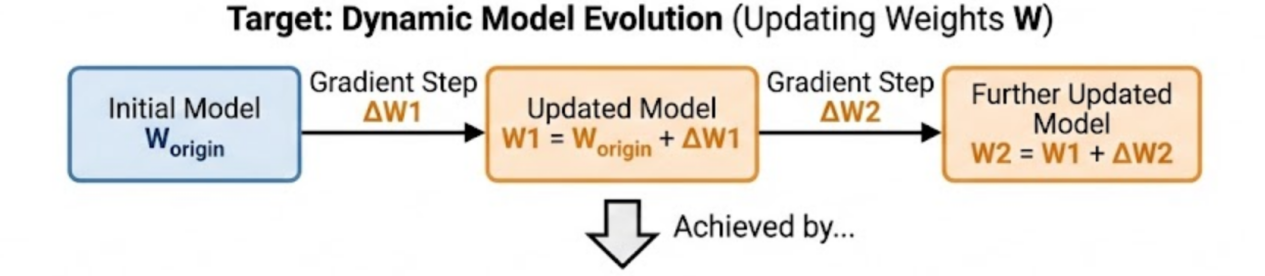
\includegraphics{images/image-0046.png}
\caption{LingBot-VA 2.0 的语义视觉-动作 tokenizer 架构}
\end{figure}

（1）视觉重建：类似VAE训练的重建损失。

（2）语义对齐：将Perception Encoder作为教师策略冻结，使得自身生成的视觉特征与之对齐，使得分词器眼中的画面从低级的像素升维成高级的语义概念。

（3）潜在动作提取：训练逆动力学模型（IDM）和前向动力学模型（FDM），前者可以从前后两帧的状态特征中提取出两帧之间采取的动作特征，后者试图用前一帧的状态特征与该动作特征还原后一帧的状态特征。该项损失旨在确保Tokenizer得到的隐变量能反映动作动态，而不仅仅是压缩像素特征。

\hypertarget{ux4e8cux8badux7ec3ux6570ux636elingbot-va-2.0}{%
\subsubsection{（二）训练数据（LingBot-VA 2.0）}\label{ux4e8cux8badux7ec3ux6570ux636elingbot-va-2.0}}

\begin{enumerate}
\def\labelenumi{\arabic{enumi}.}
\item
  通用图文视频：提供最宽的外观和动力学先验。
\item
  机器人数据：遥操作数据、AgiBot、OXE（含DROID）等。
\item
  第一人称人类视频：有65.4k个episode、3000多种场景任务组合，每帧都标了双手的6-DoF位姿和每只手22个手指关节角。人手全部对齐为平行夹爪。
\item
  后续ICL用的合成数据：先让多模态LLM做任务分析、生成图像编辑指令，把机器人首帧改写成人类操作的初始观测，再用视频生成模型合成人类操作视频，最后由一个VLM从任务语义保真和物理合理性给机器人数据和生成的人类操作视频打分，合格的才和原机器人视频配成一对。覆盖了10多个机器人视频源、5000多个任务和50000对以上的人机配对。
\end{enumerate}

\hypertarget{ux4e09ux9884ux8badux7ec3ux4efbux52a1lingbot-va-2.0}{%
\subsubsection{（三）预训练任务（LingBot-VA 2.0）}\label{ux4e09ux9884ux8badux7ec3ux4efbux52a1lingbot-va-2.0}}

T2I（文生图）：负责建立视觉语义的对齐、把潜空间和语言结合在一起。

T2V（文生视频）：从互联网规模视频里学通用的时间动力学。

TI2VA（text-image to video-action）：既预测未来潜变量，又对相邻状态之间的潜在动作做逆动力学建模。

ICL（上下文学习）：以人类演示视频为条件上下文，要求模型在不更新权重的情况下泛化生成新实例的操作轨迹。

HCT（人机协同训练）：将人类视频与机器人数据置于共享世界模型中联合训练，提取跨本体的通用动作表征。

为了更好地继承先验知识，五个训练任务全程联合优化，只随训练进度调混合权重。早期把质量集中在T2I，中期移向T2V，晚期集中到TI2VA、ICL和HCT但也对T2l、T2V等提供非零的正则，以免模型遗忘底层的世界常识。

\hypertarget{ux56dbux5f02ux6b65ux63a8ux7406}{%
\subsubsection{（四）异步推理}\label{ux56dbux5f02ux6b65ux63a8ux7406}}

整体上``块内扩散，块间自回归''，一次扩散的块可以包含若干token。将块编号为0，1，2，\ldots\ldots{}

为避免停顿，在机器人执行动作时，模型需提前预测下一个动作，即异步推理。LingBot-VA 2.0的异步推理工作流如下：

\begin{figure}[htbp]
\centering
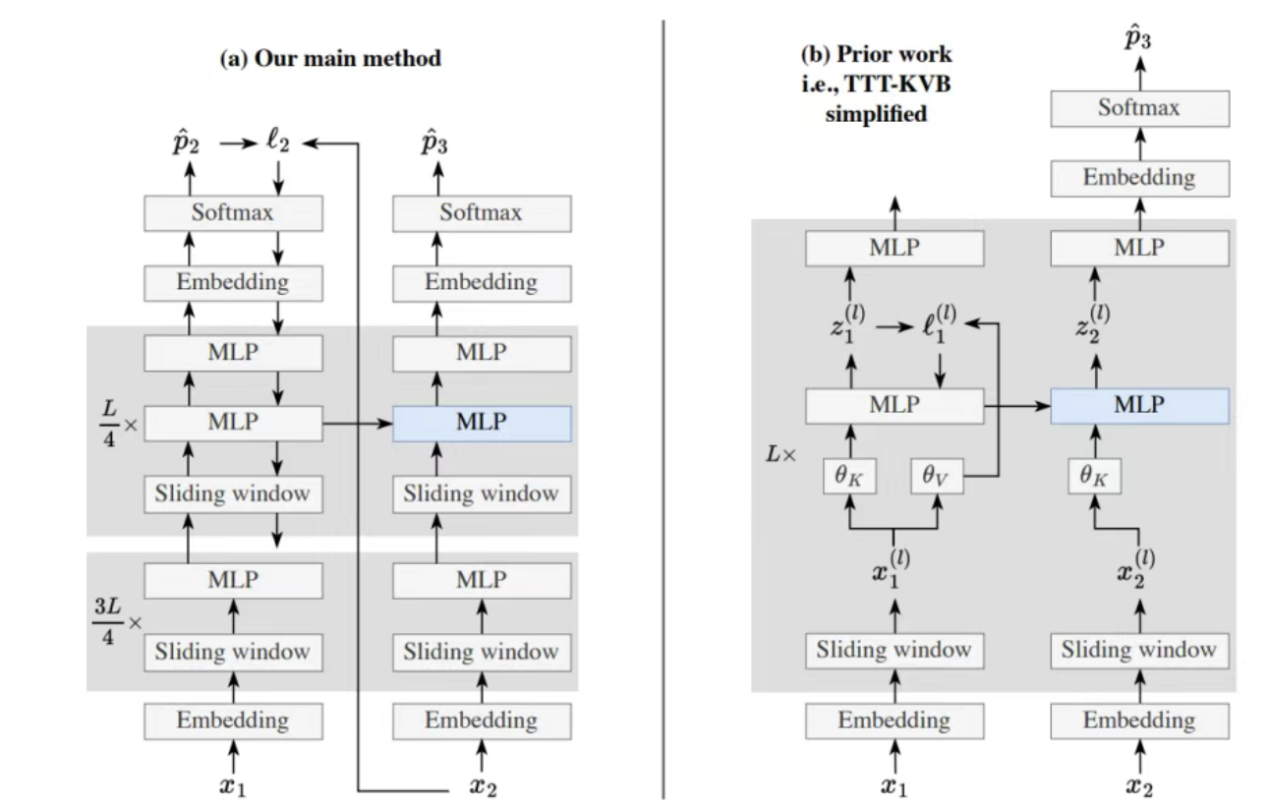
\includegraphics{images/image-0047.png}
\caption{LingBot-VA 2.0 的异步推理时间线}
\end{figure}

在动作0被预测出来后，动作0才能开始执行。模型需在动作0执行的同时，先预测状态2和动作1，此时上下文中的状态1还是预测值。如果上下文中不断积累预测值，将容易发生偏差累积。因此，在动作0执行完毕来到状态1、状态2和动作1预测完毕后，要将真实的状态1写入上下文，代替之前的预测值，这样上下文中就只有状态2是预测值，此时再执行动作1、预测状态3和动作2，以此类推，保证上下文中只有一个状态是预测值，且模型预测和动作执行可以同时进行。

\hypertarget{ux4e8cux7269ux7406tokenux7684ux7edfux4e00ux81eaux56deux5f52ux9884ux6d4b}{%
\subsection{二、物理token的统一自回归预测}\label{ux4e8cux7269ux7406tokenux7684ux7edfux4e00ux81eaux56deux5f52ux9884ux6d4b}}

具身智能中，未来视觉状态和动作本质都是高维连续信号。PAR、PhysGen等论文及NVIDIA的DreamDojo等提出了状态与策略统一编码于``物理token''中，统一进行自回归生成，再在下游解码为状态与策略输出的范式。

\hypertarget{ux4e00ux6838ux5fc3ux601dux60f3-19}{%
\subsubsection{（一）核心思想}\label{ux4e00ux6838ux5fc3ux601dux60f3-19}}

将过去的视频和动作均编码为统一的物理token。设 \(t\) 时刻的视频帧token集合为 \(o_t\)（PhysGen中每个 \(o_t\) 包含360个token），动作token集合为 \(a_t\)（PhysGen中每个 \(a_t\) 包含8个token），则上下文序列为 \([\mathrm{prompt},o_1,a_1,o_2,a_2,\ldots,o_t,a_t]\)，联合预测下一步的 \([o_{t+1},a_{t+1}]\)。预测出的 \([o_{t+1},a_{t+1}]\) 再通过扩散解码，分别得出连续的未来状态值（视频）和要采取的动作值。

具体来说， \(o_t\) 和 \(a_t\) 也不一样： \(o_t\) 内部的token可以并行生成； \(a_t\) 内部则按时间顺序严格串行，但利用Multi-token prediction的方法，在动作块内部拉长微观的规划视野。即便只预判2到3步极其微小的机械臂位姿，也能让自回归生成的动作轨迹更加连贯，有效避免控制上的``短视''和抖动。

\begin{figure}[htbp]
\centering
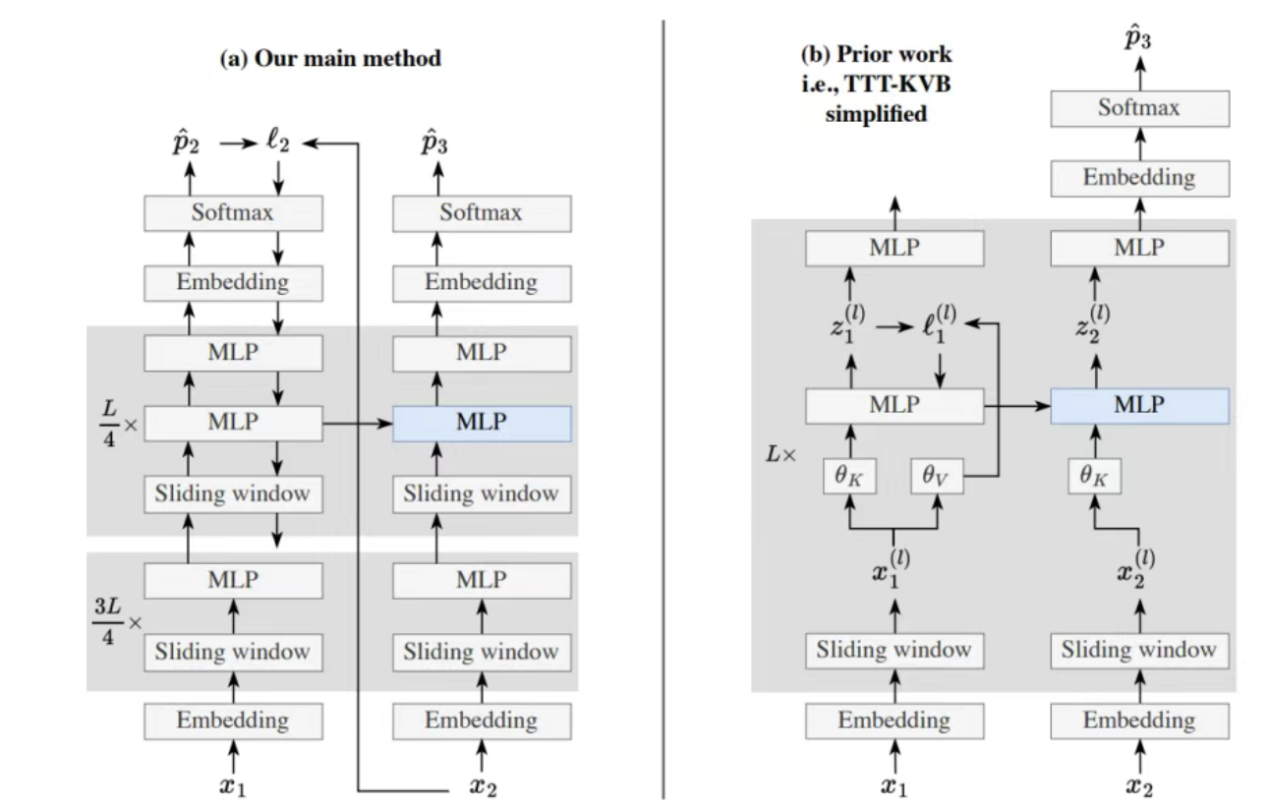
\includegraphics{images/image-0048.png}
\caption{统一物理 token 的自回归模型架构}
\end{figure}

\hypertarget{ux4e8cux81eaux56deux5f52transformer}{%
\subsubsection{（二）自回归Transformer}\label{ux4e8cux81eaux56deux5f52transformer}}

主干Transformer网络采取自回归生成范式。因果掩码方式如下：

\begin{enumerate}
\def\labelenumi{\arabic{enumi}.}
\tightlist
\item
  帧内部：块级全注意力
\end{enumerate}

对于物理token中的视频帧部分，掩码允许同一个画面内的所有图像块相互``看到''彼此。单张图像内的空间信息是同时存在的，没有时间上的先后顺序。全注意力机制能保证模型完整地提取这一帧的全局空间特征。

\begin{enumerate}
\def\labelenumi{\arabic{enumi}.}
\setcounter{enumi}{1}
\tightlist
\item
  动作内部：时间因果注意力
\end{enumerate}

对于物理标记中的动作部分，模型执行严格的时间因果掩码。在一个时间步的动作块内，各个token仍有先后顺序，时间上靠前的动作标记无法关注到排在它后面的动作标记。这是因为动作是随时间线性发生的连续序列，必须遵守``过去决定未来，未来不能干涉过去''的物理法则。

\begin{enumerate}
\def\labelenumi{\arabic{enumi}.}
\setcounter{enumi}{2}
\tightlist
\item
  动作单向关注视觉
\end{enumerate}

在同一个时间步t中，动作token被允许单向地关注视频token。这也就是让模型学会了``给定目标状态，反推所需的动作''的逆运动学推导。

\begin{enumerate}
\def\labelenumi{\arabic{enumi}.}
\setcounter{enumi}{3}
\tightlist
\item
  跨时间步：全局时间因果
\end{enumerate}

在不同的时间步之间，严格遵守时间因果掩码，用t时刻以前的信息预测t+1时刻，防止未来帧的信息泄露到过去的规划中。

\hypertarget{ux4e09ux6269ux6563ux89e3ux7801ux5668}{%
\subsubsection{（三）扩散解码器}\label{ux4e09ux6269ux6563ux89e3ux7801ux5668}}

与传统的离散分类不同，PhysGen引入了基于DiT（Diffusion Transformer）的去噪过程，利用扩散损失直接在连续空间中估计概率分布。

模型训练时对动作噪声进行预测，从而最小化均方误差损失：

\[
\mathcal{L}(P_n,Z_n)=\mathbb{E}_{\varepsilon,t}\left[\left\|\varepsilon-\varepsilon_\theta(P_{n,t}\mid t,Z_n)\right\|^2\right].
\]

推理阶段去噪的公式为：

\[
\begin{aligned}
P_{n,t-1}
&=\frac{1}{\sqrt{\alpha_t}}
\left(
P_{n,t}-\frac{1-\alpha_t}{\sqrt{1-\bar{\alpha}_t}}
\varepsilon_\theta(P_{n,t}\mid t,Z_n)
\right)
+\sigma_t\varepsilon.
\end{aligned}
\]

去噪后的物理标记最终被分离，并解码为预测的视频帧和要在物理世界中执行的机器人动作。

\hypertarget{ux56dbboa-token}{%
\subsubsection{（四）BOA token}\label{ux56dbboa-token}}

在真实的物理世界中，因果关系非常严格。假设机器人要完成一个任务：

\begin{itemize}
\tightlist
\item
  初始时刻 \(t=0\)：机器人睁开眼睛，看到桌子上的杯子，此时得到初始视觉观察结果（Frame 0）。但在这个极其短暂的瞬间，还没有执行任何动作。
\item
  第一步 \(t=1\)：模型处理Frame 0的信息，决定伸出机械臂，输出第一个动作（Action 1）。动作使物理世界发生变化，机器人随后看到新的画面（Frame 1）。
\end{itemize}

PhysGen框架将视频帧标记（Frame Token）和动作标记（Action Token）拼在一起，组成物理标记（Physical Token） \(P_n\)，其具体编码为

\[
P_n=[O_n;E_{A,n}].
\]

按照上述物理直觉，输入给模型的历史序列由两部分组成：

\begin{itemize}
\tightlist
\item
  视觉观察序列： \(\lbrace O_0,O_1,O_2,\ldots,O_{N-1}\rbrace\)，从0开始，共 \(N\) 个初始帧。
\item
  对应动作序列： \(\lbrace A_1,A_2,\ldots,A_{N-1}\rbrace\)，从1开始，共 \(N-1\) 个初始动作。
\end{itemize}

如果强行把二者打包成 \(P_n\)，就会遇到一个尴尬的时间偏移问题： \(P_0=[O_0;\mathcjk{什么都没有}]\)，而 \(P_1=[O_1;A_1]\)、 \(P_2=[O_2;A_2]\)。

为在数学结构上完美对齐这两个长度不一的序列，作者在动作序列最前面人为加入一个可学习的占位符，称为BOA（Begin of Action）Token。它使初始物理标记可以写成

\[
P_0=[O_0;\mathrm{BOA}],
\]

从而让后续每个物理标记都稳定包含一帧视觉状态和与之对应的动作标记。

\hypertarget{ux4e94ux8badux7ec3ux5de5ux4f5cux6d41}{%
\subsubsection{（五）训练工作流}\label{ux4e94ux8badux7ec3ux5de5ux4f5cux6d41}}

\begin{enumerate}
\def\labelenumi{\arabic{enumi}.}
\tightlist
\item
  预训练
\end{enumerate}

在预训练阶段，模型的主干网络仅仅在海量的视频数据上进行了训练。这个阶段模型没有见过任何机器人的动作指令，它学到的是``世界是如何运转的''（例如：杯子掉在地上会碎、手碰到物体物体会移动等纯物理和时间动态）。

这个阶段只训练了语言Tokenizer、视觉Tokenizer（3D-VAE）、自回归Transformer主干网络，以及帧生成器（Frame Diffusion），动作模块并不参与。

\begin{enumerate}
\def\labelenumi{\arabic{enumi}.}
\setcounter{enumi}{1}
\tightlist
\item
  动作微调
\end{enumerate}

为了让模型能够控制机器人，作者会在具体的下游任务上进行微调（Fine-tuning）。在这个阶段，模型会使用带有动作标签的演示数据。但是，因为模型在第一阶段已经懂得了物理世界的运作规律，它所需的动作数据量极小。

此时，模型会增加一个用于编码动作的Action Tokenizer（一个MLP），以及一个轻量级的动作解码器（Action-DiT）。微调时，模型被训练为一旦看到BOA token，后面就按``360个视频帧token+8个动作token''交替生成，系统也会按token数量交替分发给不同解码器。

\hypertarget{ux53c2ux8003ux6587ux732e-159}{%
\subsection{参考文献}\label{ux53c2ux8003ux6587ux732e-159}}

\vspace{0.25em}
\begin{itemize}
\tightlist
\item
  Li, L., Zhang, Q., Luo, Y., et al.~(2026). \href{https://arxiv.org/abs/2601.21998}{Causal World Modeling for Robot Control}. arXiv:2601.21998.（LingBot-VA）
\item
  Zhang, Q., Li, L., Zhang, L., et al.~(2026). \href{https://arxiv.org/abs/2607.08639}{Native Video-Action Pretraining for Generalizable Robot Control}. arXiv:2607.08639.（LingBot-VA 2.0）
\item
  Song, Z., Qin, S., Chen, T., Lin, L., \& Wang, G. (2025). \href{https://arxiv.org/abs/2508.09822}{Physical Autoregressive Model for Robotic Manipulation without Action Pretraining}. arXiv:2508.09822.（PAR）
\item
  Song, Z., Li, Q., Qin, S., et al.~(2026). \href{https://arxiv.org/abs/2603.00110}{Learning Physics from Pretrained Video Models: A Multimodal Continuous and Sequential World Interaction Models for Robotic Manipulation}. arXiv:2603.00110.（PhysGen）
\item
  Gao, S., Liang, W., Zheng, K., et al.~(2026). \href{https://arxiv.org/abs/2602.06949}{DreamDojo: A Generalist Robot World Model from Large-Scale Human Videos}. arXiv:2602.06949.（NVIDIA DreamDojo）
\end{itemize}

\clearpage

\hypertarget{ux63a8ux7406ux65f6ux4e0dux751fux6210ux89c6ux9891ux7684ux4e16ux754c-ux52a8ux4f5cux6a21ux578b}{%
\section{推理时不生成视频的世界-动作模型}\label{ux63a8ux7406ux65f6ux4e0dux751fux6210ux89c6ux9891ux7684ux4e16ux754c-ux52a8ux4f5cux6a21ux578b}}

\hypertarget{ux4e00ux95eeux9898ux80ccux666f-10}{%
\subsection{一、问题背景}\label{ux4e00ux95eeux9898ux80ccux666f-10}}

世界-动作模型（WAM）尽管有助于解决VLA模型存在的问题，但其必须生成未来的视频帧，导致存在明显的推理延迟。物理世界并不会停下来，因此机器人必须实现低延迟的实时控制，过长的延迟往往是不可接受的。针对此问题，如何让世界-动作模型在推理时不需要生成完整的视频成为了一个重要的研究方向。

\hypertarget{ux4e8cfast-wamux63a8ux7406ux65f6ux5f03ux7528ux89c6ux9891ux5206ux652fux4ec5ux4f7fux7528ux52a8ux4f5cux5206ux652f}{%
\subsection{二、Fast-WAM：推理时弃用视频分支、仅使用动作分支}\label{ux4e8cfast-wamux63a8ux7406ux65f6ux5f03ux7528ux89c6ux9891ux5206ux652fux4ec5ux4f7fux7528ux52a8ux4f5cux5206ux652f}}

\hypertarget{ux4e00ux6a21ux578bux67b6ux6784ux4e0eux8badux7ec3ux5de5ux4f5cux6d41}{%
\subsubsection{（一）模型架构与训练工作流}\label{ux4e00ux6a21ux578bux67b6ux6784ux4e0eux8badux7ec3ux5de5ux4f5cux6d41}}

Fast-WAM以Wan2.2作为基座模型，复用了其视频DiT、文本编码器和视频VAE，并经过后训练改造为MoT架构。

\textbf{第一步：Token的精准分组}

在送入MoT架构之前，所有输入信息被严格划分为三个Token组：

\begin{enumerate}
\def\labelenumi{\arabic{enumi}.}
\tightlist
\item
  视觉锚点 \(f_0\)：当前第一帧观测图像的``干净''潜在特征，不加噪。
\item
  未来视频 \(f_1,\ldots,f_h\)：未来视频帧的加噪潜在特征，仅在训练时存在。
\item
  动作序列 \(a_1,\ldots,a_h\)：要生成的动作块的加噪特征。
\end{enumerate}

这里的``第一帧''是相对于原本要生成的``未来视频块''而言的锚点（Anchor）。模型摒弃生成未来画面的过程，将这唯一的一帧当前图像输入视频骨干网络中进行一次单向前向传播，提取世界表征，然后直接交给动作专家网络去生成后续动作。这种设计赋予了Fast-WAM类似标准VLA的极速实时响应能力。

\textbf{第二步：全局文本Cross-Attention注入}

在这三个Token组进入DiT的每一层时，所有Token组都会通过Cross-Attention机制关注语言特征向量。数学上， \(f_0\)、 \(f_{1:h}\) 和 \(a_{1:h}\) 都作为Query，而文本特征作为Key和Value。这保证了无论是提取当前环境的视觉特征、推演未来的物理变化，还是规划机器人的具体动作，都始终受到人类语言指令的引导。

\textbf{第三步：结构化Self-Attention掩码}

注入文本信息后，Token之间在DiT内部进行自注意力交互。Video DiT和Action DiT通过严格的注意力掩码实现``组合''与``隔离''：

\begin{itemize}
\tightlist
\item
  Video DiT的内部交互：未来的加噪视频Token \(f_1,\ldots,f_h\) 可以在视频分支内双向关注，并且被允许关注第一帧干净特征 \(f_0\)，使模型能基于初始状态推演未来。
\item
  Action DiT的内部交互：动作Token \(a_1,\ldots,a_h\) 可以在动作分支内双向关注，也被允许关注第一帧干净特征 \(f_0\)，使模型能基于当前视觉状态规划连贯动作。
\item
  不可跨越的红线：动作Token绝对不允许关注未来视频Token；同时，第一帧干净Token \(f_0\) 不关注任何其他Token，以免被噪声污染。
\end{itemize}

严格隔离的根本原因是：如果训练时动作特征看到了未来视频特征，动作专家就会根据``未来已经发生的结果''反推动作，形成依赖。然而在真实部署时，为追求极低延迟，Fast-WAM会直接砍掉整个未来视频生成分支。如果模型在训练中养成了依赖未来视频的习惯，推理时一旦看不到未来视频，动作分支就会因信息缺失而崩溃。结构化掩码强迫动作预测只立足于当下，即第一帧和文本，从根本上解耦训练时的视频辅助和推理时的动作生成。

\hypertarget{ux4e8cux63a8ux7406ux5de5ux4f5cux6d41}{%
\subsubsection{（二）推理工作流}\label{ux4e8cux63a8ux7406ux5de5ux4f5cux6d41}}

推理阶段彻底抛弃显式视频生成：

\begin{enumerate}
\def\labelenumi{\arabic{enumi}.}
\tightlist
\item
  单次前向传播：仅保留第一帧的干净潜在特征，将其输入视频骨干网络进行一次单向前向传播，提取具有物理意义的潜在世界表征 \(z(o,l)\)。
\item
  直接动作去噪：动作专家DiT直接基于该表征参数化动作分布
\end{enumerate}

\[
p_\theta(a_{1:H}\mid o,l)=p_\theta(a_{1:H}\mid z(o,l)).
\]

\begin{enumerate}
\def\labelenumi{\arabic{enumi}.}
\setcounter{enumi}{2}
\tightlist
\item
  输出执行：由于不需要实例化和去噪未来视频帧，动作生成只需10步、无分类器引导（CFG=1.0）的去噪即可输出动作序列。
\end{enumerate}

\hypertarget{ux4e09ux5b9eux9a8cux7ed3ux679c}{%
\subsubsection{（三）实验结果}\label{ux4e09ux5b9eux9a8cux7ed3ux679c}}

\begin{itemize}
\tightlist
\item
  Fast-WAM的表现与显式生成未来的变体（Joint和IDM）极其接近。
\item
  如果去掉训练时的视频协同训练任务，模型在RoboTwin上的成功率骤降至83.8\%，在真机折叠毛巾任务上的成功率更断崖式跌至10\%。
\end{itemize}

因此，WAM能力增强的关键在于训练阶段的视频预测任务重塑了模型对物理世界的表征，而不在于推理阶段显式生成未来画面。Fast-WAM可以在训练时吸收世界模型带来的物理先验，同时在部署时获得类似VLA的实时响应。

\hypertarget{ux4e09dyna-2ux63a8ux7406ux65f6ux89c6ux9891ux5206ux652fux4e0dux4f5cux9884ux6d4bux53eaux4e3aux52a8ux4f5cux5206ux652fux63d0ux4f9bux89c6ux89c9-ux6587ux672cux7279ux5f81}{%
\subsection{三、Dyna-2：推理时视频分支不作预测、只为动作分支提供视觉-文本特征}\label{ux4e09dyna-2ux63a8ux7406ux65f6ux89c6ux9891ux5206ux652fux4e0dux4f5cux9884ux6d4bux53eaux4e3aux52a8ux4f5cux5206ux652fux63d0ux4f9bux89c6ux89c9-ux6587ux672cux7279ux5f81}}

Dyna-2是在大量以人类第一视角视频为核心的数据上训练的世界-动作模型，同样用视频生成和动作生成目标联合训练。关于人类第一视角视频数据的Scaling在具身数据的章节另行探讨，这里主要分析Dyna-2的模型架构。

\hypertarget{ux4e00ux6a21ux578bux67b6ux6784-2}{%
\subsubsection{（一）模型架构}\label{ux4e00ux6a21ux578bux67b6ux6784-2}}

\begin{enumerate}
\def\labelenumi{\arabic{enumi}.}
\tightlist
\item
  Video Transformer层
\end{enumerate}

输入：已观测到的视频帧Vc=\{v\_1,v\_2,\ldots,v\_N\}；待去噪的未来视频帧z\_t=\{z\_N+1,\ldots,z\_N+H\}；文本指令T。

注意力范式：视频帧之间采取因果注意力，Vc内部v\_i只能注意到v\_1,\ldots,v\_i-1；z\_t对Vc只能单向关注；视频帧对文本采取Cross Attention，以视频帧为Query，文本为Key和Value，即视频帧对应的向量从文本中吸收信息。

输出：Vc经过Video Transformer层后得到吸收了文本信息（但不吸收z\_t信息）的已观测到的视觉特征Vc'（可看成Vc和T的函数），经过1-3个Video Transformer层的视觉特征向量都会被注入Action Transformer参与动作生成（研究表明经过较少的层数就可以得到有用的视觉特征，不需要等到深层跑完）；z\_t经过Video Transformer层后得到去噪后的未来帧z\_t'（可看成Vc、z\_t和T的函数），训练时用流匹配计算视觉部分的损失。

\begin{enumerate}
\def\labelenumi{\arabic{enumi}.}
\setcounter{enumi}{1}
\tightlist
\item
  Action Transformer层
\end{enumerate}

输入：待去噪的动作块a\_t=\{a\_N+1,\ldots,a\_N+H\}；机器人本体感受量（如当前joint positions、joint velocities、gripper state、end-effector state等）；来自Video Transformer层的已观测到的视觉特征Vc'。

注意力范式：动作块a\_t内部采取双向注意力；动作块a\_t对已观测到的视觉特征Vc'采取Cross Attention，以动作为Query，视觉特征为Key和Value。动作块不直接attend文本，但通过已观测到的视觉特征Vc'可间接获取文本信息；动作块不从未来视觉预测z\_t'中获取任何信息。

输出：去噪后的动作块a\_t'既是最终推理结果，也用于训练时计算动作部分的损失

Action Transformer层数更少，推理时只需要跑各Action Transformer层和Video Transformer较浅的几层即可生成动作，保证了较高的速度。

\begin{enumerate}
\def\labelenumi{\arabic{enumi}.}
\setcounter{enumi}{2}
\tightlist
\item
  实例说明
\end{enumerate}

假设机器人已经观测到3帧 \(I_1,I_2,I_3\)，训练数据中还包含真实未来视频 \(I_4,I_5,I_6\)。未来帧先被编码为潜变量并加噪，形成 \(z_{4,t},z_{5,t},z_{6,t}\)。Video Transformer的输入可以示意为：

\begin{verbatim}
past context                  noisy future
I1  I2  I3       |        z4,t  z5,t  z6,t
        │
Video Transformer（causal attention）
        │
text ──cross-attention
        │
predicted video velocity
\end{verbatim}

Action Transformer读取的是世界模型骨干对已观测视频的表征，并输出动作；它不读取未来预测分支中的 \(z_{4,t},z_{5,t},z_{6,t}\)。也就是说，训练中的未来视频仅用于塑造世界模型表征，不会成为动作推理的必需输入。

\hypertarget{ux56dbbeing-h0.7ux8badux7ec3ux65f6ux8ba9ux52a8ux4f5cux9884ux6d4bux4e0eux57faux4e8eux672aux6765ux72b6ux6001ux7684ux52a8ux4f5cux9884ux6d4bux5bf9ux9f50}{%
\subsection{四、Being-H0.7：训练时让``动作预测''与``基于未来状态的动作预测''对齐}\label{ux56dbbeing-h0.7ux8badux7ec3ux65f6ux8ba9ux52a8ux4f5cux9884ux6d4bux4e0eux57faux4e8eux672aux6765ux72b6ux6001ux7684ux52a8ux4f5cux9884ux6d4bux5bf9ux9f50}}

\hypertarget{ux4e00ux6838ux5fc3ux601dux60f3-20}{%
\subsubsection{（一）核心思想}\label{ux4e00ux6838ux5fc3ux601dux60f3-20}}

Being-H0.7不需要在像素层面预测未来，而是直接在训练时让动作预测与基于未来状态的动作预测对齐。模型引入了一组可学习的Latent Queries，在Transformer层层前向传播的过程中，这组查询向量不断从多模态上下文中汲取与任务相关的信息，将其压缩重组、生成动作；另外在训练时，将观测到的未来状态也压缩到Latent空间，也从多模态上下文中汲取与任务相关的信息，将其压缩重组、生成动作；让前者（先验分支）向后者（后验分支）对齐。

\begin{itemize}
\tightlist
\item
  先验分支（Prior Branch）：最终用于实机部署的干线分支，仅依赖当前指令和观测，使用Latent Queries生成动作。
\item
  后验分支（Posterior Branch）：仅在训练阶段存在的辅助分支，将干线中的Latent Queries替换为由视觉编码器提取的未来观察嵌入（Future Embeddings）。
\item
  对齐机制：在隐藏层特征级别计算先验分支与后验分支的对齐损失，迫使先验分支在只看到当下画面的情况下，推断出与``看到未来''相同的特征表示。
\end{itemize}

\hypertarget{ux4e8cux8badux7ec3ux5de5ux4f5cux6d41}{%
\subsubsection{（二）训练工作流}\label{ux4e8cux8badux7ec3ux5de5ux4f5cux6d41}}

\textbf{步骤1：上下文编码与序列构建}

给定任务指令 \(x\)、时间长度为 \(H\) 的历史观测 \(o_{-H:0}\) 以及机器人本体状态 \(s\)。将这些特征映射并拼接后，在动作块 \(a_{0:T}\) 的预测序列前插入数量为 \(K\)、维度为 \(d\) 的潜在查询矩阵 \(Q\in\mathbb{R}^{K\times d}\)，构建先验分支的完整Transformer序列：

\[
S=[x;o_{-H:0};s;Q;a_{0:T}].
\]

\textbf{步骤2：后验分支的未来特征提取}

训练时同步取得未来真实观测视频帧 \(\tilde{o}_{0:T}\)，使用冻结的预训练ViT和Perceiver重采样器 \(E\)，将其压缩为大小与 \(Q\) 一致的未来嵌入：

\[
z^{\mathrm{post}}=E(\tilde{o}_{0:T})\in\mathbb{R}^{K\times d}.
\]

\textbf{步骤3：混合Transformer双分支前向传播}

为提高计算效率，算法不串行执行两次巨大的前向传播，而是用Mixture-of-Transformers架构将两个分支合并成一个长序列，并应用双分支注意力掩码（Dual-Branch Attention Mask）：两个分支都能看到共享上下文 \(c=[x;o_{-H:0};s]\)，但先验分支和后验分支的Token彼此不可见。

\textbf{步骤4：损失函数计算}

整个框架通过三组损失联合优化。

\begin{enumerate}
\def\labelenumi{\arabic{enumi}.}
\tightlist
\item
  动作流匹配损失：基于扩散生成范式，分别计算两个分支对加噪动作 \(\tilde a_t\) 的去噪速度场损失。若真实动作为 \(a\)、加噪时间为 \(t\)，目标速度为 \(u_t=a-\tilde a_t\)，则
\end{enumerate}

\[
\mathcal{L}_{\mathrm{FM}}^{\mathrm{prior}}=\left\|v_\theta^{\mathrm{prior}}(a_t,c)-u_t\right\|_2^2,
\]

\[
\mathcal{L}_{\mathrm{FM}}^{\mathrm{post}}=\left\|v_\theta^{\mathrm{post}}(a_t,c,z^{\mathrm{post}})-u_t\right\|_2^2.
\]

\begin{enumerate}
\def\labelenumi{\arabic{enumi}.}
\setcounter{enumi}{1}
\tightlist
\item
  隐状态联合对齐损失：在第 \(l\) 个包含对齐的Transformer层，提取先验分支隐状态 \(h_l^{\mathrm{prior}}\) 与后验分支隐状态 \(h_l^{\mathrm{post}}\)，计算均方误差：
\end{enumerate}

\[
\mathcal{L}_{\mathrm{align}}=\frac{1}{L}\sum_{l=1}^{L}\left\|h_l^{\mathrm{prior}}-h_l^{\mathrm{post}}\right\|_2^2.
\]

\begin{enumerate}
\def\labelenumi{\arabic{enumi}.}
\setcounter{enumi}{2}
\tightlist
\item
  防崩溃正则化损失：为防止对齐导致隐特征趋于全0或方向单一，分别施加范数与秩的惩罚。范数正则化为
\end{enumerate}

\[
\mathcal{R}_{\mathrm{norm}}(h)=\left[\operatorname{ReLU}\!\left(\tau-\|h\|_2\right)\right]^2.
\]

秩正则化由Gram矩阵 \(G\) 的归一化特征值 \(p_i\) 的信息熵表示：

\[
\mathcal{R}_{\mathrm{rank}}(H)=\sum_{i=1}^{B}p_i\log p_i.
\]

\hypertarget{ux4e09ux63a8ux7406ux5de5ux4f5cux6d41}{%
\subsubsection{（三）推理工作流}\label{ux4e09ux63a8ux7406ux5de5ux4f5cux6d41}}

由于模型将特征对齐与前向生成解耦，推理阶段非常轻量：

\begin{enumerate}
\def\labelenumi{\arabic{enumi}.}
\tightlist
\item
  观察采集：机器人摄像头实时采集当前画面，处理并拼接为上下文向量。
\item
  纯先验分支执行：完全丢弃庞大的后验分支和所有未来视频输入，只保留Transformer骨干、Latent Queries \(Q\) 以及用于扩散的Flow Matching生成头。
\item
  动作块输出与UAC异步控制：模型一次性生成连续的未来动作块 \(a_{0:T}\)。真实系统部署时结合通用异步分块机制（UAC），服务器异步推理未来动作序列，机器人驱动器从线程安全缓冲池持续取出历史前缀锁定动作执行。二者解耦后，以约3至4毫秒每步的延迟实现平滑动态控制。
\end{enumerate}

\hypertarget{ux53c2ux8003ux6587ux732e-160}{%
\subsection{参考文献}\label{ux53c2ux8003ux6587ux732e-160}}

\vspace{0.25em}
\begin{itemize}
\tightlist
\item
  Yuan, T., Dong, Z., Liu, Y., \& Zhao, H. (2026). \href{https://arxiv.org/abs/2603.16666}{Fast-WAM: Do World Action Models Need Test-time Future Imagination?}. arXiv:2603.16666.
\item
  Dyna Robotics. (2026). \href{https://www.dyna.co/dyna-2}{Dyna-2: A 1-Million-Hour Scaling Law for World-Action Models}. Official research report.
\item
  Luo, H., Zhang, W., Feng, Y., et al.~(2026). \href{https://arxiv.org/abs/2605.00078}{Being-H0.7: A Latent World-Action Model from Egocentric Videos}. arXiv:2605.00078.
\end{itemize}

\clearpage

\hypertarget{ux89e6ux89c9ux7684ux5efaux6a21}{%
\section{触觉的建模}\label{ux89e6ux89c9ux7684ux5efaux6a21}}

\hypertarget{ux4e00ux89e6ux89c9ux5efaux6a21ux7684ux96beux70b9}{%
\subsection{一、触觉建模的难点}\label{ux4e00ux89e6ux89c9ux5efaux6a21ux7684ux96beux70b9}}

\begin{enumerate}
\def\labelenumi{\arabic{enumi}.}
\item
  缺少获取大规模的触觉数据的方法。目前行业内可获得的有效触觉数据远远少于语言、视觉等数据。且带触觉的采集设备依旧存在较高的门槛，数据采集规模化难度较大。
\item
  触觉模态与语言、视觉模态融合建模难度大。触觉通常发生在机器人与物体接触的瞬间，具有高频性；而在其他时间可能又不存在此信号，具有稀疏性。这决定了触觉模态不能简单粗暴地和与语言、视觉模态数据混合在一起。
\item
  跨触觉传感器迁移困难。触觉传感器类型多样，可以分为视触觉、压阻、电容等，所产生的信号模态不同，有图像型、阵列型、状态型等，分辨率不同，难以通用。
\item
  不同类型的末端传感器分布不同。如夹爪和灵巧手的触觉传感器的分布和数量等都不同，但它们又要作用于同一套机器人策略，增大了建模的难度，尤其是对于机器人全身的策略进行建模的难度。
\end{enumerate}

\hypertarget{ux4e8cux89e6ux89c9ux5efaux6a21ux7684ux4e3bux8981ux65b9ux6cd5}{%
\subsection{二、触觉建模的主要方法}\label{ux4e8cux89e6ux89c9ux5efaux6a21ux7684ux4e3bux8981ux65b9ux6cd5}}

\hypertarget{ux4e00ux89e6ux89c9ux6a21ux578bux4e0eux4e3bux5e72ux7b56ux7565ux76f8ux5bf9ux5206ux5f00}{%
\subsubsection{（一）触觉模型与主干策略相对分开}\label{ux4e00ux89e6ux89c9ux6a21ux578bux4e0eux4e3bux5e72ux7b56ux7565ux76f8ux5bf9ux5206ux5f00}}

这种方法把触觉做成独立的高频纠错模块，附加在主干策略之外。如CraftNet把一台机器人拆成三个异步运转的部分。System0是一个每秒上百次的交互环节，专门接收力和力矩信号，在接触的瞬间实时微调指尖位置。触觉在这里是反应最快的纠偏回路。

\begin{figure}[htbp]
\centering
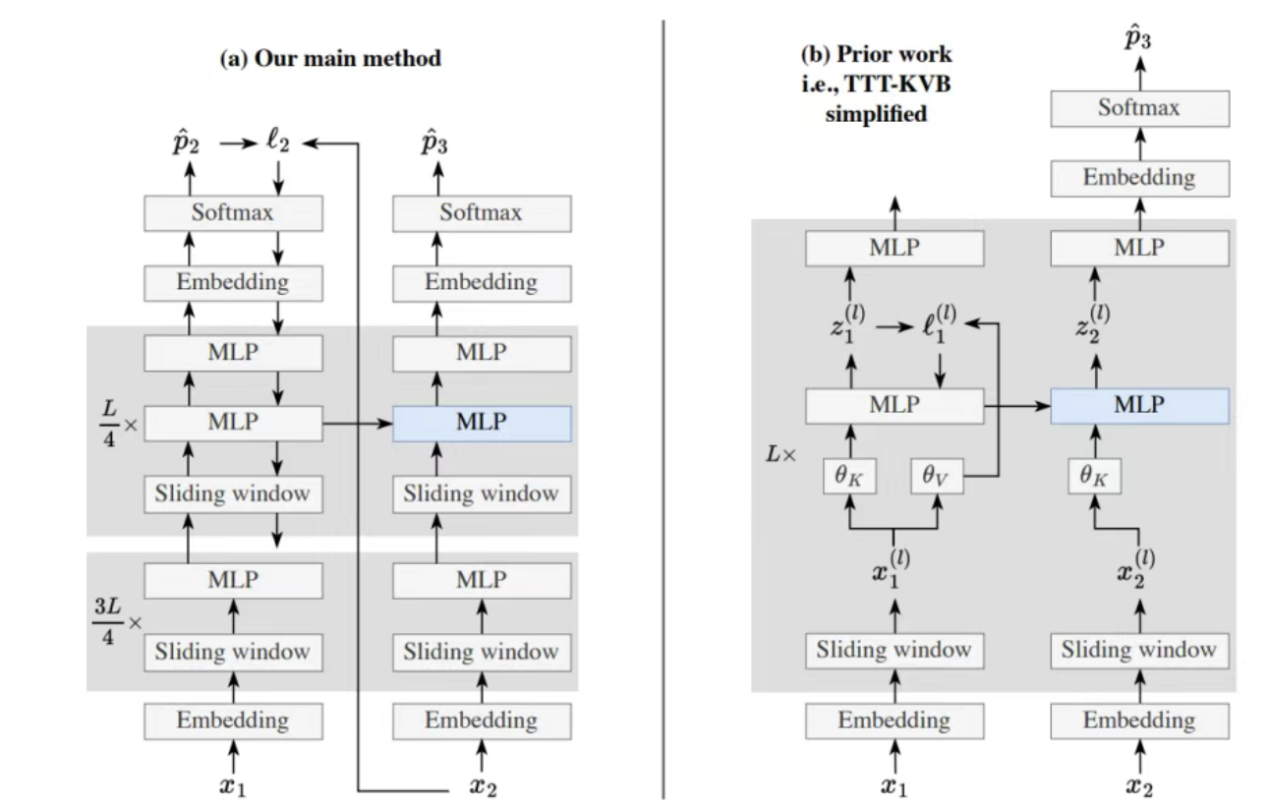
\includegraphics{images/image-0049.png}
\caption{CraftNet 中触觉模型与主干策略分开的架构}
\end{figure}

但分层架构的缺点在于，触觉并没有进入主干模型的预训练，Scaling潜力不如端到端统一，且无法实现跨本体复用。

\hypertarget{ux4e8cux7528adapterux63a5ux5165ux4e3bux5e72ux7b56ux7565}{%
\subsubsection{（二）用Adapter接入主干策略}\label{ux4e8cux7528adapterux63a5ux5165ux4e3bux5e72ux7b56ux7565}}

以Tactile-VLA为例，用一个adapter把触觉token注入视觉语言模型，和视觉、语言模态共享注意力，并不另起炉灶。这种方法的优点在于，可以让视觉信息进入主干策略，实现了端到端统一，避免了分层架构固有的弊端。

\begin{figure}[htbp]
\centering
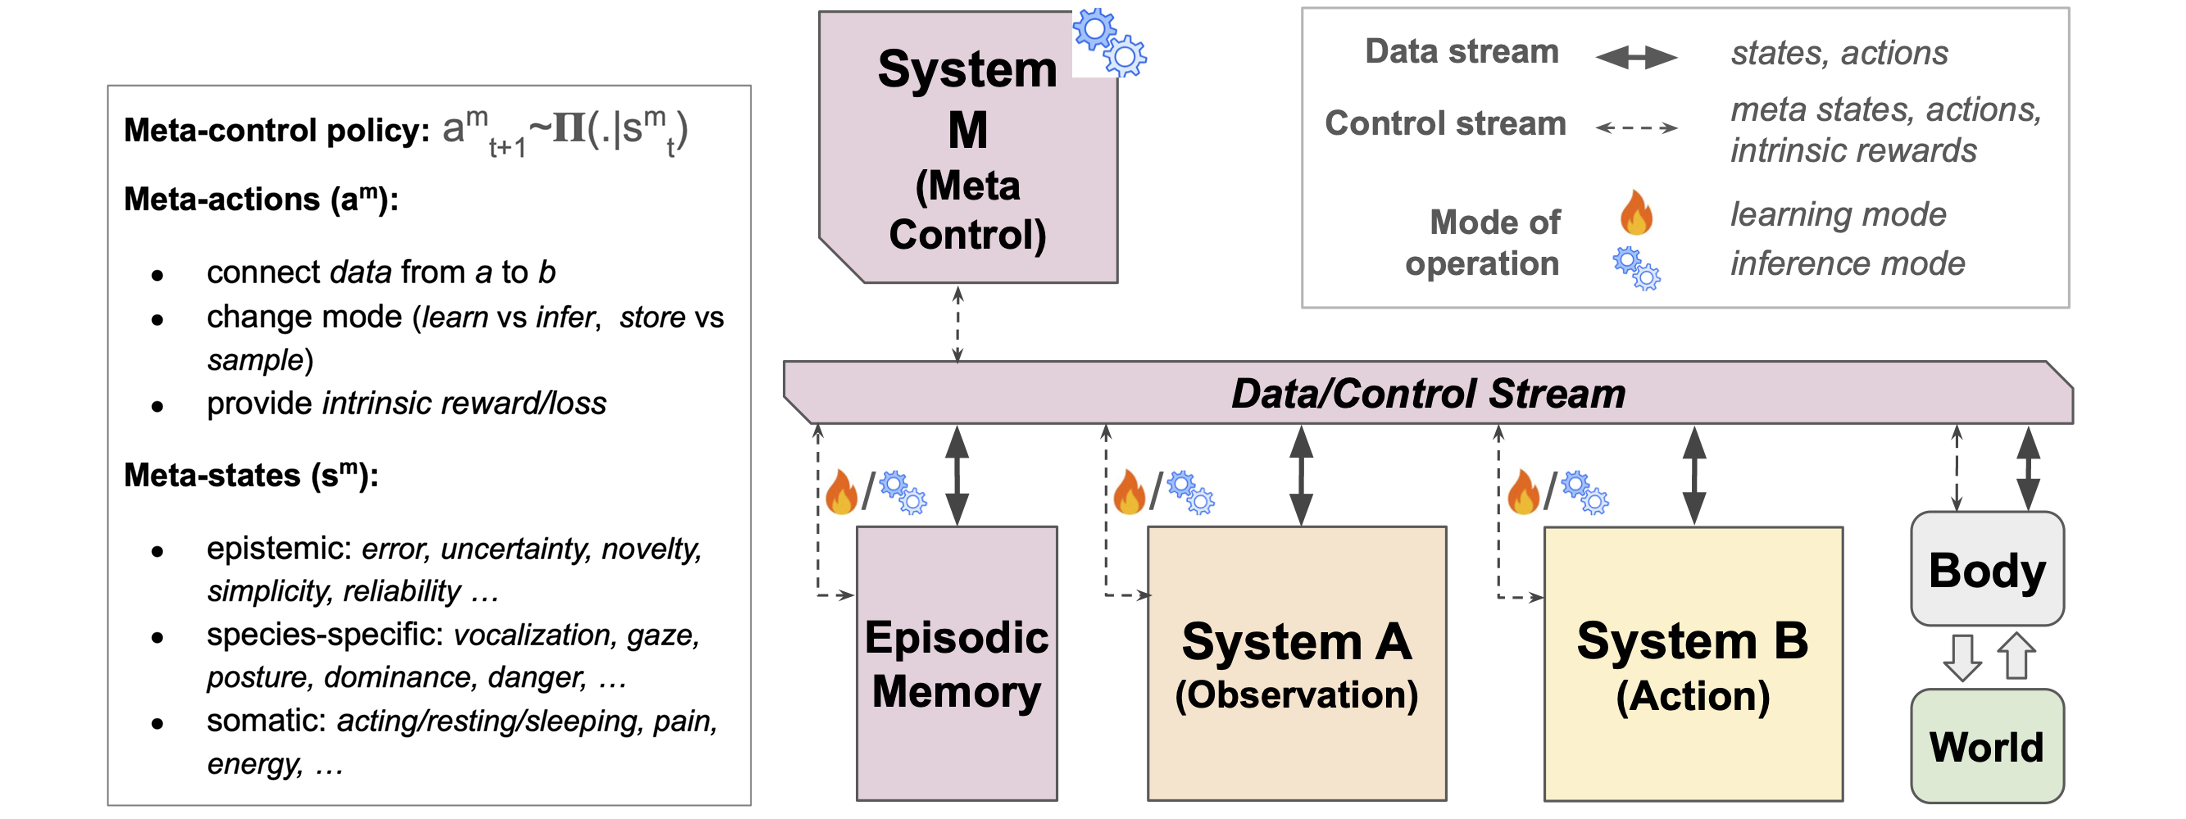
\includegraphics{images/image-0050.png}
\caption{Tactile-VLA 通过 Adapter 接入主干策略的架构}
\end{figure}

但仍存在两个缺点：

\begin{enumerate}
\def\labelenumi{\arabic{enumi}.}
\item
  对于已经训练完毕的视觉语言模型，后续接入触觉信息微调时，触觉和已有的视觉语言知识之间容易互相干扰。事实上，如果不对触觉做恰当的模态融合，强行和视觉语言合并在一起，触觉非但帮不上忙，反而会干扰视觉语言感知，连累整体性能。
\item
  依然绑定在单一传感器上，传感器一旦更换，整个Adapter将无法复用。
\end{enumerate}

\hypertarget{ux4e09ux5728ux4e3bux5e72ux7b56ux7565ux6a21ux578bux4e2dux7528moeux533aux5206ux4e0dux540cux6a21ux6001}{%
\subsubsection{（三）在主干策略模型中用MoE区分不同模态}\label{ux4e09ux5728ux4e3bux5e72ux7b56ux7565ux6a21ux578bux4e2dux7528moeux533aux5206ux4e0dux540cux6a21ux6001}}

可通过混合专家模型，用门控来控制不同阶段的主导专家，如无接触时以视觉为主，接触时触觉的权重显著增强。如ForceVLA把力读数投影成token，在动作解码的阶段用一个力觉MoE做模态和阶段感知的路由；ForceVLA2一边把力当成文本提示喂进VLM形成``力觉任务概念''，一边在动作端上跨尺度进行MoE。

运用MoE的好处在于两个方面：

\begin{enumerate}
\def\labelenumi{\arabic{enumi}.}
\item
  由于触觉和视觉、语言模态的特点相差较大，用不同权重隔离可避免伤害预训练获得的视觉语言知识。
\item
  只要规定好触觉输入数据格式，就支持在微调时将预训练得到的共享触觉专家复用到从没有见过的传感器。只需要训练一个轻量级编码器，将传感器的数据转换为触觉专家可读取的格式即可。
\end{enumerate}

\hypertarget{ux4e09ftp-1ux878dux5408ux89e6ux89c9ux5efaux6a21ux7684ux57faux7840ux6a21ux578b}{%
\subsection{三、FTP-1：融合触觉建模的基础模型}\label{ux4e09ftp-1ux878dux5408ux89e6ux89c9ux5efaux6a21ux7684ux57faux7840ux6a21ux578b}}

\hypertarget{ux4e00ux89e6ux89c9ux4f20ux611fux5668ux7684ux6570ux636eux683cux5f0fux89c4ux5b9a}{%
\subsubsection{（一）触觉传感器的数据格式规定}\label{ux4e00ux89e6ux89c9ux4f20ux611fux5668ux7684ux6570ux636eux683cux5f0fux89c4ux5b9a}}

论文《FTP-1: A Generalist Foundation Tactile Policy Across Tactile Sensors for Contact-Rich Manipulation》提出了数据接口MTTS。其坐标用手本身的功能区划分，把一只手划分成24个功能区，任何传感器的触觉信号都按功能区归位，从而可以翻译成同一套槽位token。每个token都会有功能区embedding标明感觉来自哪一个功能区。

\hypertarget{ux4e8cux4e0dux540cux7c7bux578bux4f20ux611fux5668ux4fe1ux53f7ux7684ux7ffbux8bd1ux65b9ux6cd5}{%
\subsubsection{（二）不同类型传感器信号的翻译方法}\label{ux4e8cux4e0dux540cux7c7bux578bux4f20ux611fux5668ux4fe1ux53f7ux7684ux7ffbux8bd1ux65b9ux6cd5}}

图像型（形变图）：训练轻量级ViT处理图像，转换为符合MTTS格式的token。

阵列型（压力网格）：训练轻量级CNN提取特征，转换为符合MTTS格式的token。

状态型（力读数）：先用傅里叶编码，再训练轻量级MLP变换数据格式，转换为符合MTTS格式的token。

\hypertarget{ux4e09ux6a21ux578bux67b6ux6784}{%
\subsubsection{（三）模型架构}\label{ux4e09ux6a21ux578bux67b6ux6784}}

\begin{figure}[htbp]
\centering
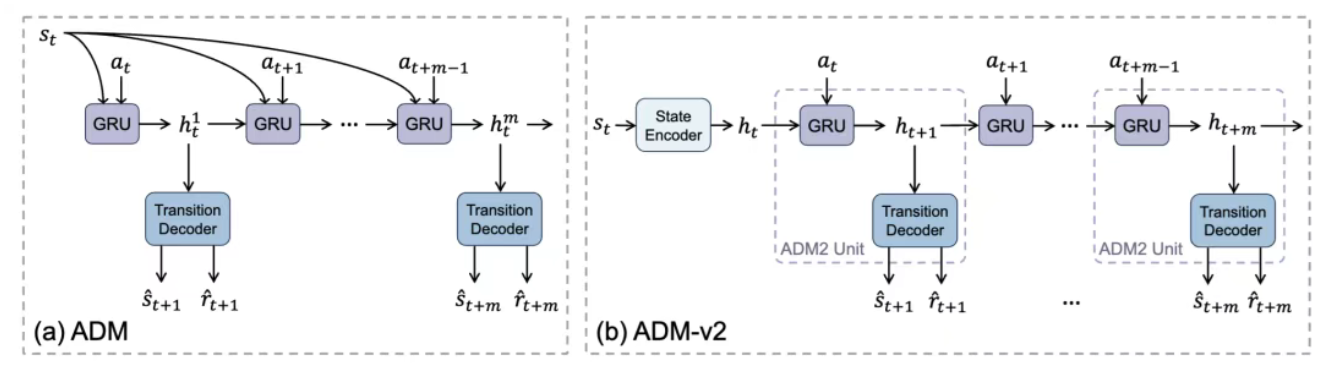
\includegraphics{images/image-0051.png}
\caption{FTP-1 触觉基础模型架构}
\end{figure}

不同类型传感器信号经过翻译后进入主干模型。主干模型主要由视觉语言、动作和触觉专家构成，视觉语言专家具备VLM的能力，动作专家用流匹配方法生成连续动作，触觉专家处理触觉信号。动作专家可以从触觉专家中单向获取信息。

\hypertarget{ux53c2ux8003ux6587ux732e-161}{%
\subsection{参考文献}\label{ux53c2ux8003ux6587ux732e-161}}

\vspace{0.25em}
\begin{itemize}
\tightlist
\item
  Sharpa. (2026). \href{https://www.sharpa.com/blogs/news/sharpa-announces-craftnet-a-hierarchical-vtla-model-for-fine-manipulation}{Sharpa Announces CraftNet: A Hierarchical VTLA Model for Fine Manipulation}. Official technical article.
\item
  Huang, J., Wang, S., Lin, F., Hu, Y., Wen, C., \& Gao, Y. (2025). \href{https://arxiv.org/abs/2507.09160}{Tactile-VLA: Unlocking Vision-Language-Action Model's Physical Knowledge for Tactile Generalization}. arXiv:2507.09160.
\item
  Yu, J., Liu, H., Yu, Q., et al.~(2025). \href{https://arxiv.org/abs/2505.22159}{ForceVLA: Enhancing VLA Models with a Force-aware MoE for Contact-rich Manipulation}. arXiv:2505.22159.
\item
  Li, Y., Zhaxizhuoma, Jiang, H., et al.~(2026). \href{https://arxiv.org/abs/2603.15169}{ForceVLA2: Unleashing Hybrid Force-Position Control with Force Awareness for Contact-Rich Manipulation}. arXiv:2603.15169.
\item
  Yuan, C., Zhang, Z., Zhou, M., et al.~(2026). \href{https://arxiv.org/abs/2606.13102}{FTP-1: A Generalist Foundation Tactile Policy Across Tactile Sensors for Contact-Rich Manipulation}. arXiv:2606.13102.
\item
  具身纪元. (2026). \href{https://www.jintiankansha.com/t/DWG4NegaMt}{触觉需要自己的基础模型和Open-X Embodiment}. 微信公众号文章.
\end{itemize}

\clearpage
